% ---
% Capitulo de estudo de viabilidade
% ---
\chapter{Estudo de viabilidade}

\section{Trabalhos relacionados}

\subsection{Análise crítica}

\section{Coleta de dados}

Para o levantamento de dados deste projeto foram escolhidos os instrumentos de questionário com potenciais usuários e entrevista com especialista.

\subsection{Questionário aplicado a idosos}

O principal instrumento para coleta de dados utilizado no projeto de interface foi um questionário aplicado a alunos de um curso de informática para idosos, oferecido por um grupo de pesquisa do ICMC/USP. O objetivo deste questionário foi tentar entender alguns aspectos do cotidiano deles, para poder introduzir o aplicativo de forma adequada, bem como projetar a interface móvel de modo menos intrusivo possível, respeitando condições de privacidade.

Com a ajuda dos instrutores do curso, ao final da última aula e após uma rápida apresentação das propostas desta pesquisa e objetivos do aplicativo, o questionário foi aplicado de forma online para os alunos que aceitaram a participação. 

O modelo do questionário aplicado pode ser conferido no anexo X.

\subsubsection{Resultados}

\subsection{Entrevista com especialista em gerontologia}

\subsubsection{Plano de Entrevista} \label{plano_de_entrevista}

Para o planejamento da entrevista com a especialista, foram levantados previamente os principais tópicos a serem abordados e que poderiam auxiliar na condução da pesquisa. Tais como:

\begin{itemize}
    \item Quais as carências e limitações que surgem com o envelhecimento. Exemplos: problemas de memória, dificuldades motoras, carência afetiva, prática de lazer, saudosismo, contato familiar entre outros assuntos onde um assistente tecnológico pode contribuir.
    \item Quais os desafios comportamentais no momento de oferecer cuidados especiais a idosos? Como costumam responder a alguém lhes dizendo o que fazer.
    \item Como é a familiaridade dos idosos com dispositivos tecnológicas e quais as limitações na interação.
    \item Como é a aceitação tecnológica e que tipos de metáforas podem ajudas nas tarefas.
\end{itemize}

A partir disso, foram elaboradas quatro sugestões de perguntas que serviram de guia para a condução da entrevista. 

\begin{enumerate}
    \item No contexto de um assistente tecnológico para auxiliar idosos, que tipo de limitações físicas ou problemas psicoafetivos recorrentes no envelhecimento poderiam se beneficiar? (Memória? Dificuldades motoras? Solidão?)
    \item Os idosos se sentem confortáveis quando são lembrados ou tem sua atenção chamada, seja por um assistente ou um cuidador, ou se sentem invadidos?
    \item Como os idosos de hoje tem assimilado ou aderido à tecnologia?  Ainda há muita resistência ou dificuldade de uso?
    \item A adoção de uma metáfora física, como um boneco, pode ajudar?
    \item Como geralmente são usados esses diários e lembretes? Se ele puder gravar a anotação com a própria voz, isso pode ajudar?
    \item Imaginando que o idoso vai interagir com o boneco, de quem deve partir a inciativa? Se o boneco iniciar a interação o idoso irá responder bem?
    \item Que peculiaridades do comportamento de um idoso devem ser consideradas quando se pensa em um assistente tecnológico para auxiliá-las?
\end{enumerate}

\subsection{A entrevista}

A entrevista com a Profa. Dra. Paula Costa Castro foi realizada via \emph{Skype} e gravada. Foi utilizada a abordagem semi-estruturada, onde as perguntas elencadas em \ref{plano_de_entrevista} serviram como guias, porém a entrevista foi conduzida em formato livre, explorando com mais profundidade questões sobre o envelhecimento, suas características e as alternativas a serem exploradas com apoio da tecnologia.

Sobre o envelhecimento, Paula caracterizou-o como bastante heterogêneo, tendo início pouco após os 30 anos e intensificando-se com o tempo. Explicou que os processos de condição de saúde negativa ou que podem levar a uma deficiência se iniciam das mais variadas formas desde a vida adulta. “Existe uma gama grande de problemas que podem ou não se tornar limitações funcionais”.

Dentre as questões mais relevantes para intervenções, citou o isolamento, a comunicação e o apoio para atividades.

Em relação a assimilação da tecnologia pelos idoso, Paula afirmou existirem dois perfis: os mais receptivos (digital engaged) e os menos receptivos (digital disengaged). 


\subsection{Questionário aplicado a cuidadores de idosos}

\section{Canvas}

\begin{figure}[h]
\centering
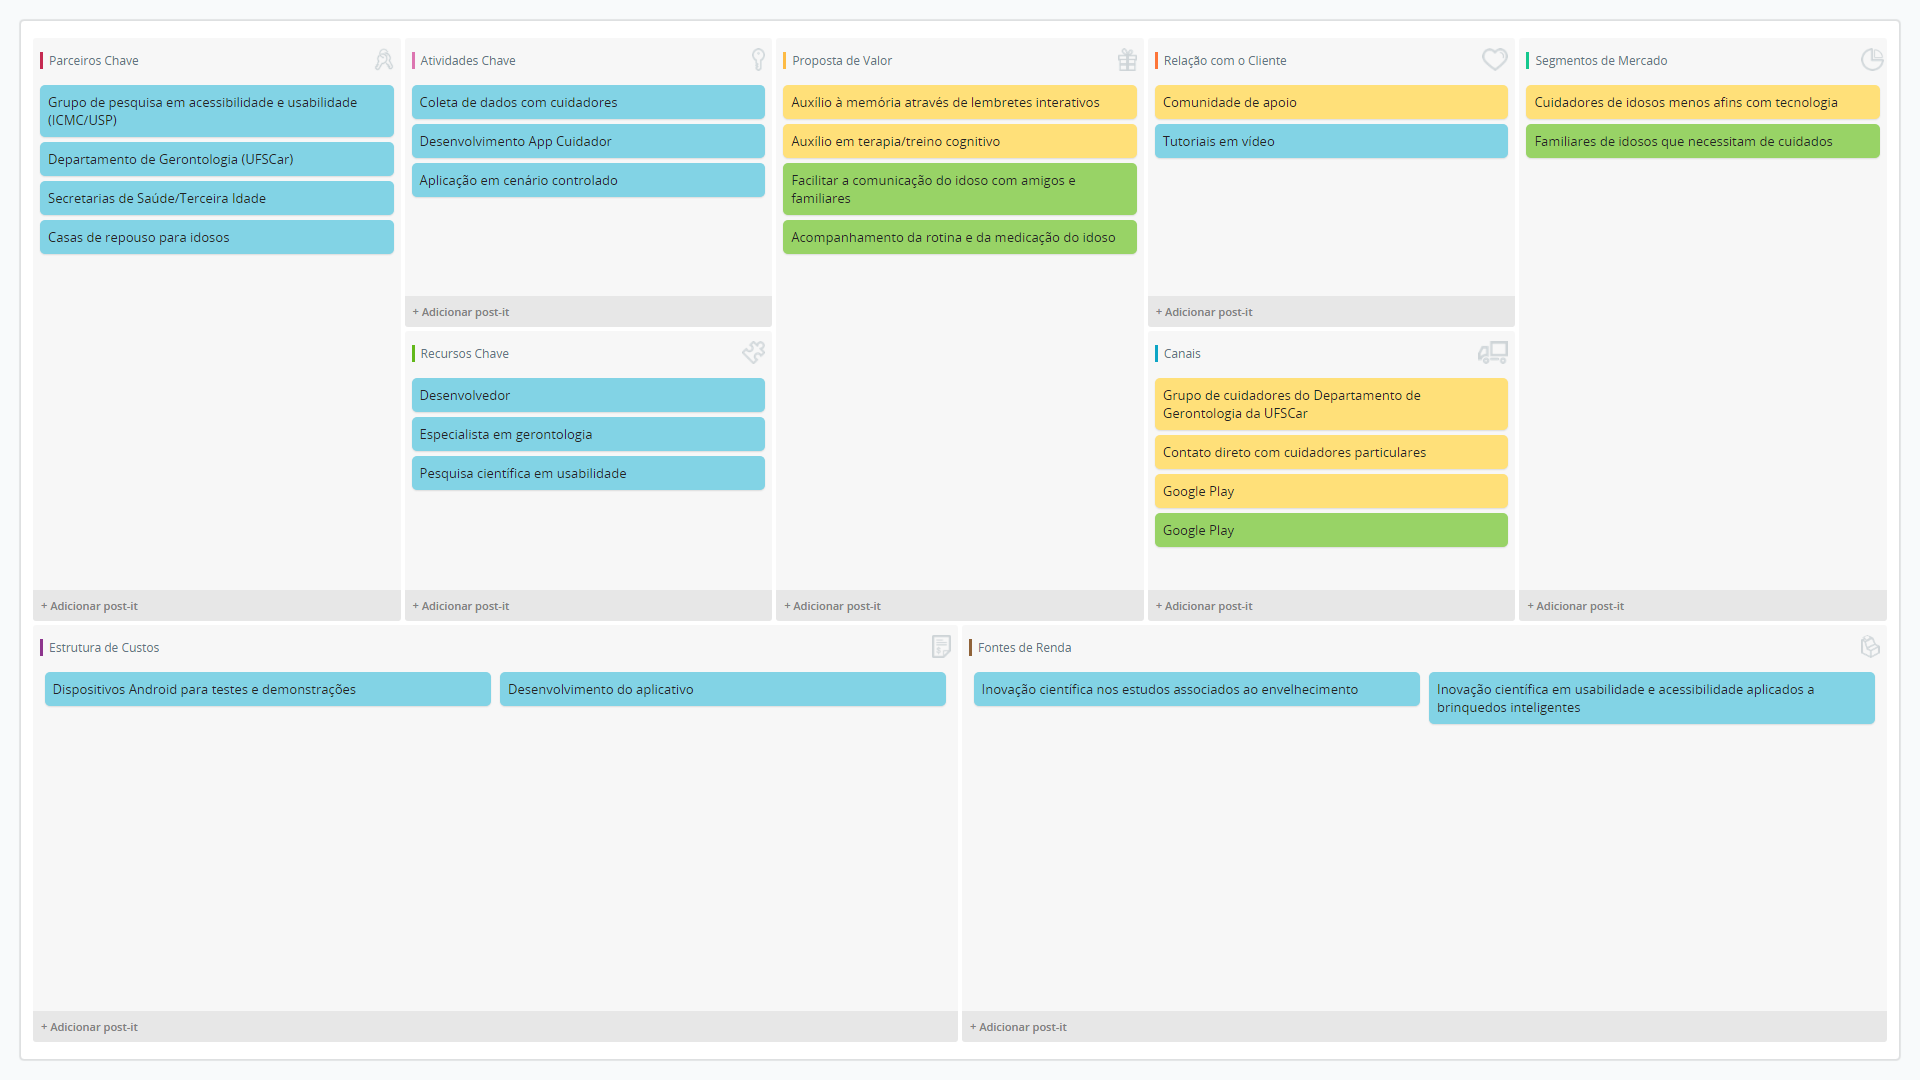
\includegraphics[width=1\textwidth]{canvas.png}
\caption{Canvas do projeto Cuidador}
\end{figure}


\section{Matriz de valor}

\begin{figure}[h]
\centering
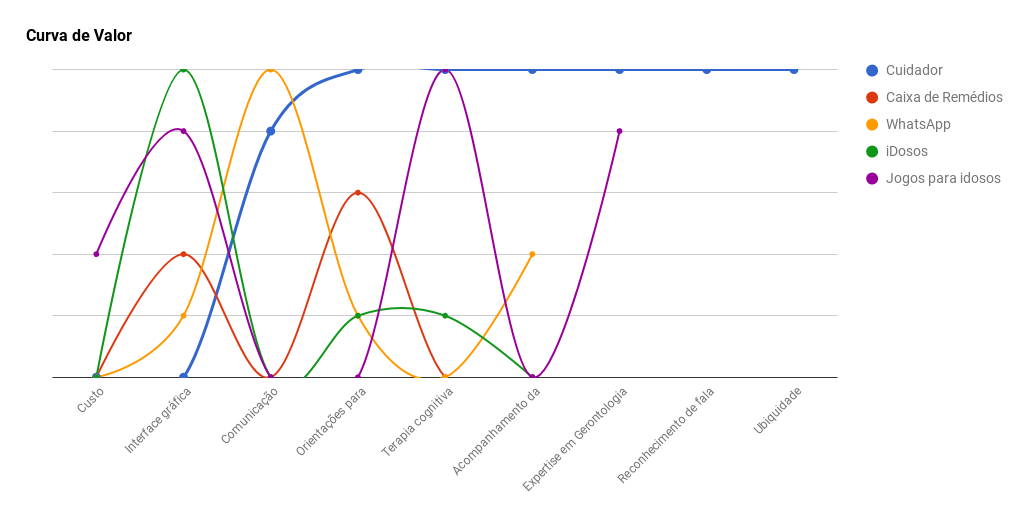
\includegraphics[width=1\textwidth]{curva.png}
\caption{Curva de valor do projeto Cuidador}
\end{figure}